%\documentclass[a4paper]{article}
\documentclass[11pt]{extarticle}

\usepackage[utf8]{inputenc}
\usepackage{listings}
\usepackage{lipsum}
\usepackage{hyperref}
\usepackage[english]{babel}
\usepackage[numbered,framed]{matlab-prettifier}
\usepackage[useregional]{datetime2}
\usepackage{graphicx}

\lstset{
  style              = Matlab-editor,
  basicstyle         = \mlttfamily,
  escapechar         = ",
  mlshowsectionrules = true,
}

\title{\vspace{2cm}Elaborato di\\ \textbf{Calcolo Numerico}\\ Anno Accademico 2016/2017\vspace{1cm}}

\author{Gabriele Puliti - \texttt{5300140} - \href{mailto:gabriele.puliti@stud.unifi.it}{\textit{gabriele.puliti@stud.unifi.it}}
\and Luca Passaretta - \texttt{ } - \href{mailto: }{\textit{ }}}

\date{}

\addto\captionsenglish{\renewcommand{\contentsname}{Capitoli}}

\begin{document}

\maketitle

\begin{center}
\today{}
\end{center}

\newpage
\
\newpage

\tableofcontents
\newpage
\
\newpage

\section{\textbf{Capitolo 1}}
\subsection{Esercizio 1}
Sapendo che il metodo iterativo è convergente a \( x^* \) allora per definizione si ha:
 \[
	\lim_{k \to +\infty}\ x_k = x^*
\]
 inoltre per definizione di \( \Phi \) si calcola il limite:
\[
    \lim_{k \to +\infty} \Phi(x_k) = \lim_{k \to +\infty} x_{k+1} = x^*
\]
 infine ipotizzando che la funzione \( \Phi \) sia uniformemente continua, è possibile calcolare il limite:
\[
    \lim_{k \to +\infty} \Phi(x_k) = \Phi(\lim_{k \to +\infty} x_k) = \Phi(x^*)
\]
 dai due limiti si ha la tesi:
\[
    \Phi(x^*) = x^* 
\]
\subsection{Esercizio 2}
Dal momento che le variabili intere di 2 byte in Fortran vengono gestite in Modulo e Segno, la variabile \texttt{n}, inizializzata con

\begin{lstlisting}
integer*2 n
\end{lstlisting}
varia tra \( - 2^{15} \leq n \leq 2^{15} - 1 \) e quindi tra  \( -32768 \leq n \leq 32767 \). \\
Andando quindi ad eseguire la somma \( (32767+1)_{10} = (0111111111111111 + 1)_{2,MS} = \\
= (11111111111111111)_{2,MS} = (-327628)_{10} \)

\subsection{Esercizio 3}
Per definizione si ha che la precisione di macchina \(u\), per arrotondamento e' data da:
\[
u=\frac{1}{2} b ^{1-m}
\]
Se \(b=8, m=5\) si ha:
\[ 
u = \frac{1}{2}\cdot 8^{1-5} = \frac{1}{2}\cdot 8^{-4} = 1,2 \cdot 10^{-4} 
\]

\subsection{Esercizio 4}
Il codice seguente:
\lstinputlisting[language=Matlab]{cap_1/es4/es4.m}
restituisce questo risultato (assumendo che $f(x)$ = $ e^x $ e $ x_0 = 0 $ ): 
\begin{center}
\begin{tabular}{c|c}
h & \( \Psi_{h}(0) \)  \\
\hline
    \(10^{-1}\) & 1.051709180756477e+00\\
    \(10^{-2}\) & 1.005016708416795e+00\\
    \(10^{-3}\) & 1.000500166708385e+00\\
    \(10^{-4}\) & 1.000050001667141e+00\\
    \(10^{-5}\) & 1.000005000006965e+00\\
    \(10^{-6}\) & 1.000000499962184e+00\\
    \(10^{-7}\) & 1.000000049433680e+00\\
    \(10^{-8}\) & 9.999999939225290e-01\\
    \(10^{-9}\) & 1.000000082740371e+00\\
    \(10^{-10}\) & 1.000000082740371e+00\\
    \(10^{-11}\) & 1.000000082740371e+00\\
    \(10^{-12}\) & 1.000088900582341e+00\\
\end{tabular} \\
\end{center}
si può notare che al diminuire del valore h, la funzione \(\Psi_{h}(0)\) approssima con maggior precisione il valore $f'(0)$, come si può vedere dal plot \ref{fes14}.
\subsection{Esercizio 5}
Tesi:\\
Sia f(x) una funzione sufficentemente regolare e h>0 una quantità ``piccola''\\
Ipotesi:\\
\[
\frac{f(x_0 + h) - f(x_0 + h)}{2h} = f'(x_0) + O(h^2)
\]
\[
\frac{f(x_0 + h) -2f(x_0) - f(x_0 + h)}{h^2} = f''(x_0) + O(h^2)
\]

Dimostrazione:\\
Sviluppiamo la funzione f(x) mediante il polinomio di taylor al secondo ordine\\
\[
f(x) = f(x_0) + (x-x_0)f'(x_0)+\frac{(x-x_0)^2}{2}f''(x_0) + O((x-x_0)^3)
\]
Sostituiamo \[x=(x_0 +h)\] e  \[x=(x_0-h)\]
\[
f((x_0 +h) = f(x_0) + hf'(x_0)+\frac{h^2}{2}f''(x_0) + O(h^3)
\]
\[
f((x_0 -h) = f(x_0) - hf'(x_0)+\frac{h^2}{2}f''(x_0) + O(h^3)
\]
Risostituendo  nel rapporto incrementale dell'ipotesi otteniamo:
\[
\frac{ f(x_0) + hf'(x_0)+\frac{h^2}{2}f''(x_0) + O(h^3) - f(x_0) - hf'(x_0)+\frac{h^2}{2}f''(x_0) + O(h^3)}{2h} = \frac{2hf'(x_0) + O(h^3)}{2h} =f'(x_0) + O(h^2)
\]

Per la seconda uguaglianza dell'ipotesi basterà applicare lo stesso procedimento con uno sviluppo di taylor al 3° ordine.
\subsection{Esercizio 6}
Il codice MatLab, indicando con x=$x_n$ e r=$\epsilon$:
\lstinputlisting[language=Matlab]{cap_1/es6/es6.m}
\newpage
restituisce i valori:
\begin{center}
\begin{tabular}{c|c|c}
n & $x_n$ & $\epsilon$ \\
\hline
    0 & 2.00000000000000e+000 & 585.786437626905e-003\\
    1 & 1.50000000000000e+000 & 85.7864376269049e-003\\
    2 & 1.42857142857143e+000 & 14.3578661983335e-003\\
    3 & 1.41463414634146e+000 & 420.583968367971e-006\\
    4 & 1.41421568627451e+000 & 2.12390141496321e-006\\
    5 & 1.41421356268887e+000 & 315.774073555986e-012\\
    6 & 1.41421356237310e+000 & 0.00000000000000e+000\\
    7 & 1.41421356237310e+000 & 0.00000000000000e+000\\
\end{tabular}
\end{center}
I valori indicano che per valori di $n$ superiori a 5 l'errore, indicato con $\epsilon$, è dell'ordine di \(10^{-12}\).
\subsection{Esercizio 7}
Sapendo che la rappresentazione del numero è stata fatta usando l'arrotondamento, la precisione di macchina si calcola:
\[
u = \frac{b^{1-m}}{2}
\]
il cui valore sappiamo essere pari a:
\[
u \approx 4.66 \cdot 10^{-10}
\]
dato che stiamo cercando il numero di cifre binarie allora si deve avere $b=2$, è quindi possibile ricavare $m$:
\[
m = 1- log_2{(4.66 \cdot 10 ^{-10})} \approx 31.99
\]
possiamo pertanto affermare che servono 32 cifre dedicate alla mantissa per rappresentare il numero con precisione macchina \(4.66 \cdot 10^{-10}\).
\subsection{Esercizio 8}
Sapendo che la mantissa in decimale è calcolabile tramite la funzione:
\begin{itemize}
\item \( m = 1- log_{10}{u} \) (troncamento) 
\item \( m = 1- log_{10}{(2\cdot u)} \) (arrotondamento)
\end{itemize}
e che la precisione di macchina assuma un valore accettabilemente piccolo in modo tale che il \(log_{10}{u} \approx 1\), cioè $0<=u<1$, allora è possibile scrivere:
\begin{itemize}
\item \( m = 1 - log_{10}{u} \approx -log_{10}{u} \) (troncamento)
\item \( m = 1 - log_{10}{2u} = 1 - log_{10}{2} - log_{10}{u} \approx -log_{10}{u} \) (arrotondamento)
\end{itemize}
\subsection{Esercizio 9}
\lstinputlisting[language=Matlab]{cap_1/es9/es9.m}
Il valore di delta è uguale a \(\frac{1}{10}\), la rappresentazione binaria di questo numero però non è esatta.
Si tratta di una rappresentazione periodica e quindi, in decimale, sarà circa 0.0999, prendendo quindi $delta\approx0.9$ vedremo che per $i=10$ $x\approx0.999$, mentre per $i=11$  $x\approx1,0989$. Per questo motivo la condizione x=1 non si avvererà mai e il programma non terminerà.
\subsection{Esercizio 10}
Il calcolo della radice e dell'elevamento a potenza è sempre ben condizionato.  La parte problematica è l'overflow della somma.
Troviamo quindi il massimo dei due addendi:\\
\begin{equation}
m = max\{|x|,|y|\} 
\end{equation}
\begin{equation}
\sqrt{x^2 + y^2}
\end{equation}
Dividiamo entrambi i membri per il massimo
\begin{equation}
\sqrt{m^2*(\frac{x}{m}^2 + \frac{y}{m}^2)}
\end{equation}
Portiamo fuori il massimo dalla radice
\begin{equation}
m*\sqrt{\frac{x}{m}^2 + \frac{y}{m}^2}
\end{equation}

\subsection{Esercizio 11}
L'espressione aritmetica dei due algoritmi è:\\
\begin{itemize}
\item{1)} (x+y)+z = x+y+z 
\item{2)}  x+(y+z) = x+y+z 
\end{itemize}
Ne consegue che sono equivalenti
In aritmetica finita, invece, avremo:
\begin{itemize}
\item{1)} \( (x\oplus y)\oplus z = fl(fl(fl(x) + fl(y)) +fl(z)) = \)\\
\( =((x(1+\varepsilon_x) + y(1+\varepsilon_y))(1+\varepsilon_A) +z(1+\varepsilon_z))(1+\varepsilon_B) = \) \\
\[\varepsilon_R =\frac{(x(1+\varepsilon_x)(1+\varepsilon_A)(1+\varepsilon_B) + y(1+\varepsilon_y)(1+\varepsilon_A)(1+\varepsilon_B)+z(1+\varepsilon_z))(1+\varepsilon_B) -x-y-z}{z+y+z}     \]
prendo \( \varepsilon_M = max\{\varepsilon_x, \varepsilon_y, \varepsilon_z, \varepsilon_A, \varepsilon_B\}\)
\[\varepsilon_R \leq \frac{x(1+\varepsilon_M)^3 + y(1+\varepsilon_M)^3+z(1+\varepsilon_M)^2 -x-y-z}{z+y+z} = \]
\[ =  \frac{x(3\varepsilon_M + 3\varepsilon_M^2 +\varepsilon_M^3) + y(3\varepsilon_M + 3\varepsilon_M^2 +\varepsilon_M^3)+z(2\varepsilon_M + \varepsilon_M^2)}{z+y+z}    \]
Sapendo che \(\varepsilon_M \leq 1 \) posso affermare che \( \varepsilon_M \geq \varepsilon_M^2 \geq \varepsilon_M?3 \) ed effettuare un'altra minorazione

\[ \varepsilon_R \leq \frac{7x\varepsilon_M + 7y\varepsilon_M + 3z\varepsilon_M}{x+y+z} = \varepsilon_M(3+4\frac{x+y}{x+y+z}) \]

\item{2)}  \( x\oplus (y\oplus z) =fl(fl(x) +fl( fl(y) +fl(z)))     \) \\
Il procedimento sarà analogo a quello visto prima con lo scambio degli addendi al nominatore della frazione
\[ \varepsilon_R \leq \frac{7z\varepsilon_M + 7y\varepsilon_M + 3x\varepsilon_M}{x+y+z} = \varepsilon_M(3+4\frac{z+y}{x+y+z}) \]
\end{itemize}
\subsection{Esercizio 12}
Ipotesi: k sia il numero di condizionamento di:
\[
y = \sqrt{x}
\]
Tesi:
\[
k=\frac{1}{2}
\]
\[
f(x) = \sqrt{x}
\]
\[
f'(x) = \frac{1}{2\sqrt{x}}
\]
\[
k \equiv |f'(x) \cdot \frac{x}{y} | = | \frac{1}{2\sqrt{x}} \cdot \frac{x}{ \sqrt{x} } | = | \frac{1}{2} \cdot \frac{x}{x} | = | \frac{1}{2}|
\]
\[ \blacksquare \]

\subsection{Esercizio 13}
Il problema è che stiamo rappresentando dei numeri reali in un calcolatore quindi la loro rappresentazione comporta delle approssimazioni. Nella riga 11 abbiamo calcolato e restituito in output il valore interno al logaritmo $\big|3(1-\frac{3}{4})+1\big|$ che teoricamente è zero, ma si ottiene $ 2.220446049250313e-16 $. 
Si può vedere che il codice MatLab:
\lstinputlisting{cap_1/es13/es13.m}
calcola i valori della funzione ottenendo il grafico \ref{fes113} e si può notare che l'asintoto verticale in $x=\frac{4}{3}$ viene rappresentato come minimo della funzione $f(x)$.


\section{\textbf{Capitolo 2}}
\subsection{Esercizio 1}
Per ricercare la radice quadrata di un numero è possibile sfruttare una modifica al problema delle radici di una funzione. Infatti partendo da $x=\sqrt{\alpha}$ è possibile svilupparla trovando una funzione $f(x)$ utilizzabile nel metodo di Newton:
\[
x = \sqrt{\alpha} 
\]
\[
x^{2} = \big(\sqrt{\alpha}\big)^{2} 
\]
\[
x^{2} - \alpha = 0
\]
possiamo quindi considerare $f(x) = x^{2} - \alpha$ e $f'(x) = 2\cdot x$ . La procedura iterativa è definita quindi da:
\[
x_{n+1} = x_{n} - \frac{f(x_{n})}{f'(x_{n})} = x_{n}-\frac{x_{n}^2-\alpha}{2\cdot x_{n}} = x_{n} - \frac{x_{n}}{2} + \frac{\alpha}{2\cdot x_{n}} = \frac{x_{n}}{2}+\frac{\alpha}{2\cdot x_{n}} = \frac{1}{2} \cdot \Big(x_{n}+\frac{\alpha}{x_{n}}\Big)
\]
che ci permette di implementare il seguente script matlab e la funzione y = NewtonSqrt(alpha, x\_0, imax, tol):
\lstinputlisting[language=matlab]{cap_2/es1/es1.m}
Che restituisce in output valori che abbiamo rappresentato nella tabella seguente:
\begin{center}
\begin{tabular}{|c|c|}
\hline
$i$ & \( x_i \) \\
\hline
1 & 1.750000000000000e+00 \\
2 & 1.732142857142857e+00 \\
3 & 1.732050810014727e+00 \\
4 & 1.732050807568877e+00 \\
\hline
\end{tabular}\\
\end{center}
\subsection{Esercizio 2}
\begin{flushleft}
E' possibile effettuare gli stessi passaggi dell'esercizio precedente, ricordandosi che la radice in questo caso non è quadrata ma ennesima:
\[
x = \sqrt[n]{\alpha} 
\]
\[
x^{n} = \big(\sqrt[n]{\alpha}\big)^{n} 
\]
\[
x^{n} - \alpha = 0
\]
consideriamo quindi la funzione $f(x) = x^{n} - \alpha$ e $f'(x) = n\cdot x^{n-1}$ . La procedura iterativa è definita quindi da:
\[
x_{n+1} = x_{n} - \frac{f(x_{n})}{f'(x_{n})} = x_{n}-\frac{x_{n}^n-\alpha}{n\cdot x_{n}^{n-1}} = x_{n} - \frac{x_{n}}{n} + \frac{\alpha}{n\cdot x_{n}^{n-1}} = 
\]
\[
= \Big((n-1)\cdot x_n- \frac{\alpha}{x_n^{n-1}}\Big) \cdot \frac{1}{n} = \frac{\Big( (n-1)\cdot x_n^{n}+\alpha\Big)}{n\cdot x_n^{n-1}}
\]
La radice da approssimare in questo caso ha grado ennesimo quindi sono necessarie delle modifiche alla funzione matlab usata nell'esercizio precedente che chiamiamo y = NewtonSqrt(n, alpha, x\_0, imax, tol). Lo script MatLab corrispondente ai casi $n = 3,4,5$ è il seguente:
\lstinputlisting[language=Matlab]{cap_2/es2/es2.m}
Mostriamo l'output in forma tabellare con $i$ che rappresenta le iterazioni del metodo e $x_i$ i relativi risultati:
\begin{center}
\begin{tabular}{|c|c|c|c|}
\hline
i & $x_i$ con $n=3$ & $x_i$ con $n=4$ & $x_i$ con $n=5$\\
\hline
1 & 1.631784138709347e+00 & 1.771797299323380e+00 & 1.943788863498140e+00 \\
2 & 1.463411989089094e+00 & 1.463688102853308e+00 & 1.597060655491283e+00 \\
3 & 1.442554125137959e+00 & 1.336940995805593e+00 & 1.369877122538772e+00 \\
4 & 1.442249634601091e+00 & 1.316557487370408e+00 & 1.266284124539191e+00 \\
5 & 1.442249570307411e+00 & 1.316074279204018e+00 & 1.246387399421677e+00 \\
6 & ------------ & 1.316074012952573e+00 & 1.245731630753065e+00 \\
7 & ------------ & ------------ & 1.245730939616284e+00 \\
\hline
\end{tabular}
\end{center}
\end{flushleft}
\subsection{Esercizio 3}
Per confrontare il metodo delle secanti con quello di Newton abbiamo creato il codice MatLab:
\lstinputlisting[language=matlab]{cap_2/es3/es3.m}
I risultati ottenuti dall'utilizzo del metodo delle secanti sono: \newline
\\
\scalebox{0.9} {
\begin{tabular}{c|c|c|c|c}
i & metodo di Newton & metodo delle secanti & \big|newton-$\sqrt{2}$\big| & \big|secanti-$\sqrt{2}$\big|\\
\hline
1 & 1.750000000000000e+00 & 1.736842105263158e+00 & 3.357864376269049e-01 & 3.226285428900628e-01 \\
2 & 1.732142857142857e+00 & 1.732142857142857e+00 & 3.179292947697618e-01 & 3.179292947697618e-01 \\
3 & 1.732050810014727e+00 & 1.732050934706042e+00 & 3.178372476416318e-01 & 3.178373723329468e-01 \\
4 & --------- & 1.732050807572255e+00 & ------- & 3.178372451991598e-01\\
\end{tabular}
}
\\ \newline
Si nota dalla tabella che \( \big|newton-\sqrt{2}\big| \approx  \big|secanti-\sqrt{2}\big| \), cioè che l'ordine di grandezza dell'errore assoluto tra i due metodi è lo stesso. Si può quindi affermare che l'uso del metodo di Newton o del metodo delle secanti è equivalente.

\subsection{Funzioni MatLab Usate}
\label{functcap2}
\subsubsection{Metodo Newton per $\sqrt{\alpha}$}
\lstinputlisting[language=matlab]{cap_2/NewtonSqrt.m}
\subsubsection{Metodo Newton per $\sqrt[n]{\alpha}$}
\lstinputlisting[language=matlab]{cap_2/NewtonSqrtN.m}
\subsubsection{Metodo delle secanti per $\sqrt{\alpha}$}
\lstinputlisting[language=matlab]{cap_2/SecSqrt.m}
\subsubsection{Metodo di Newton}
\lstinputlisting[language=matlab]{cap_2/Newton.m}
\subsubsection{Metodo di Newton Modificato}
\lstinputlisting[language=matlab]{cap_2/NewtonMod.m}
\subsubsection{Metodo di accelerazione di Aitken}
\lstinputlisting[language=matlab]{cap_2/Aitken.m}
\subsubsection{Metodo delle secanti}
\lstinputlisting[language=matlab]{cap_2/secanti.m}
\subsubsection{Metodo delle corde}
\lstinputlisting[language=matlab]{cap_2/corde.m}
\subsubsection{Metodo della bisezione}
\lstinputlisting[language=matlab]{cap_2/bisect.m}
\newpage

\pagenumbering{roman}
\section{\textbf{Grafici}}
\subsection{Esercizio 1.4}
\begin{figure}[h]
\caption{Esercizio 1.4}
\label{fes14}
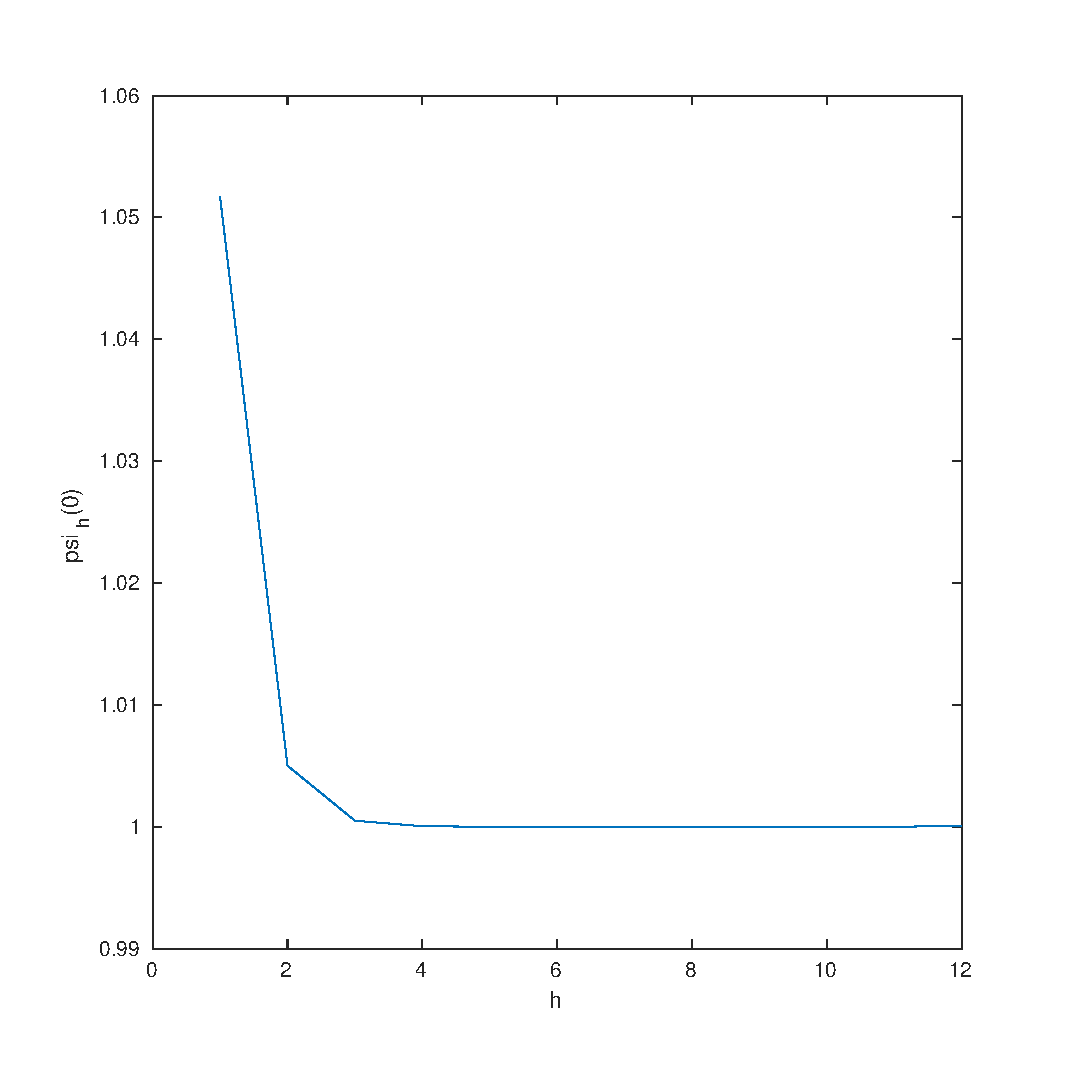
\includegraphics[width=\textwidth]{plot/fes14}
\end{figure}
\subsection{Esercizio 1.13}
\begin{figure}[h]
\caption{Esercizio 1.13}
\label{fes113}
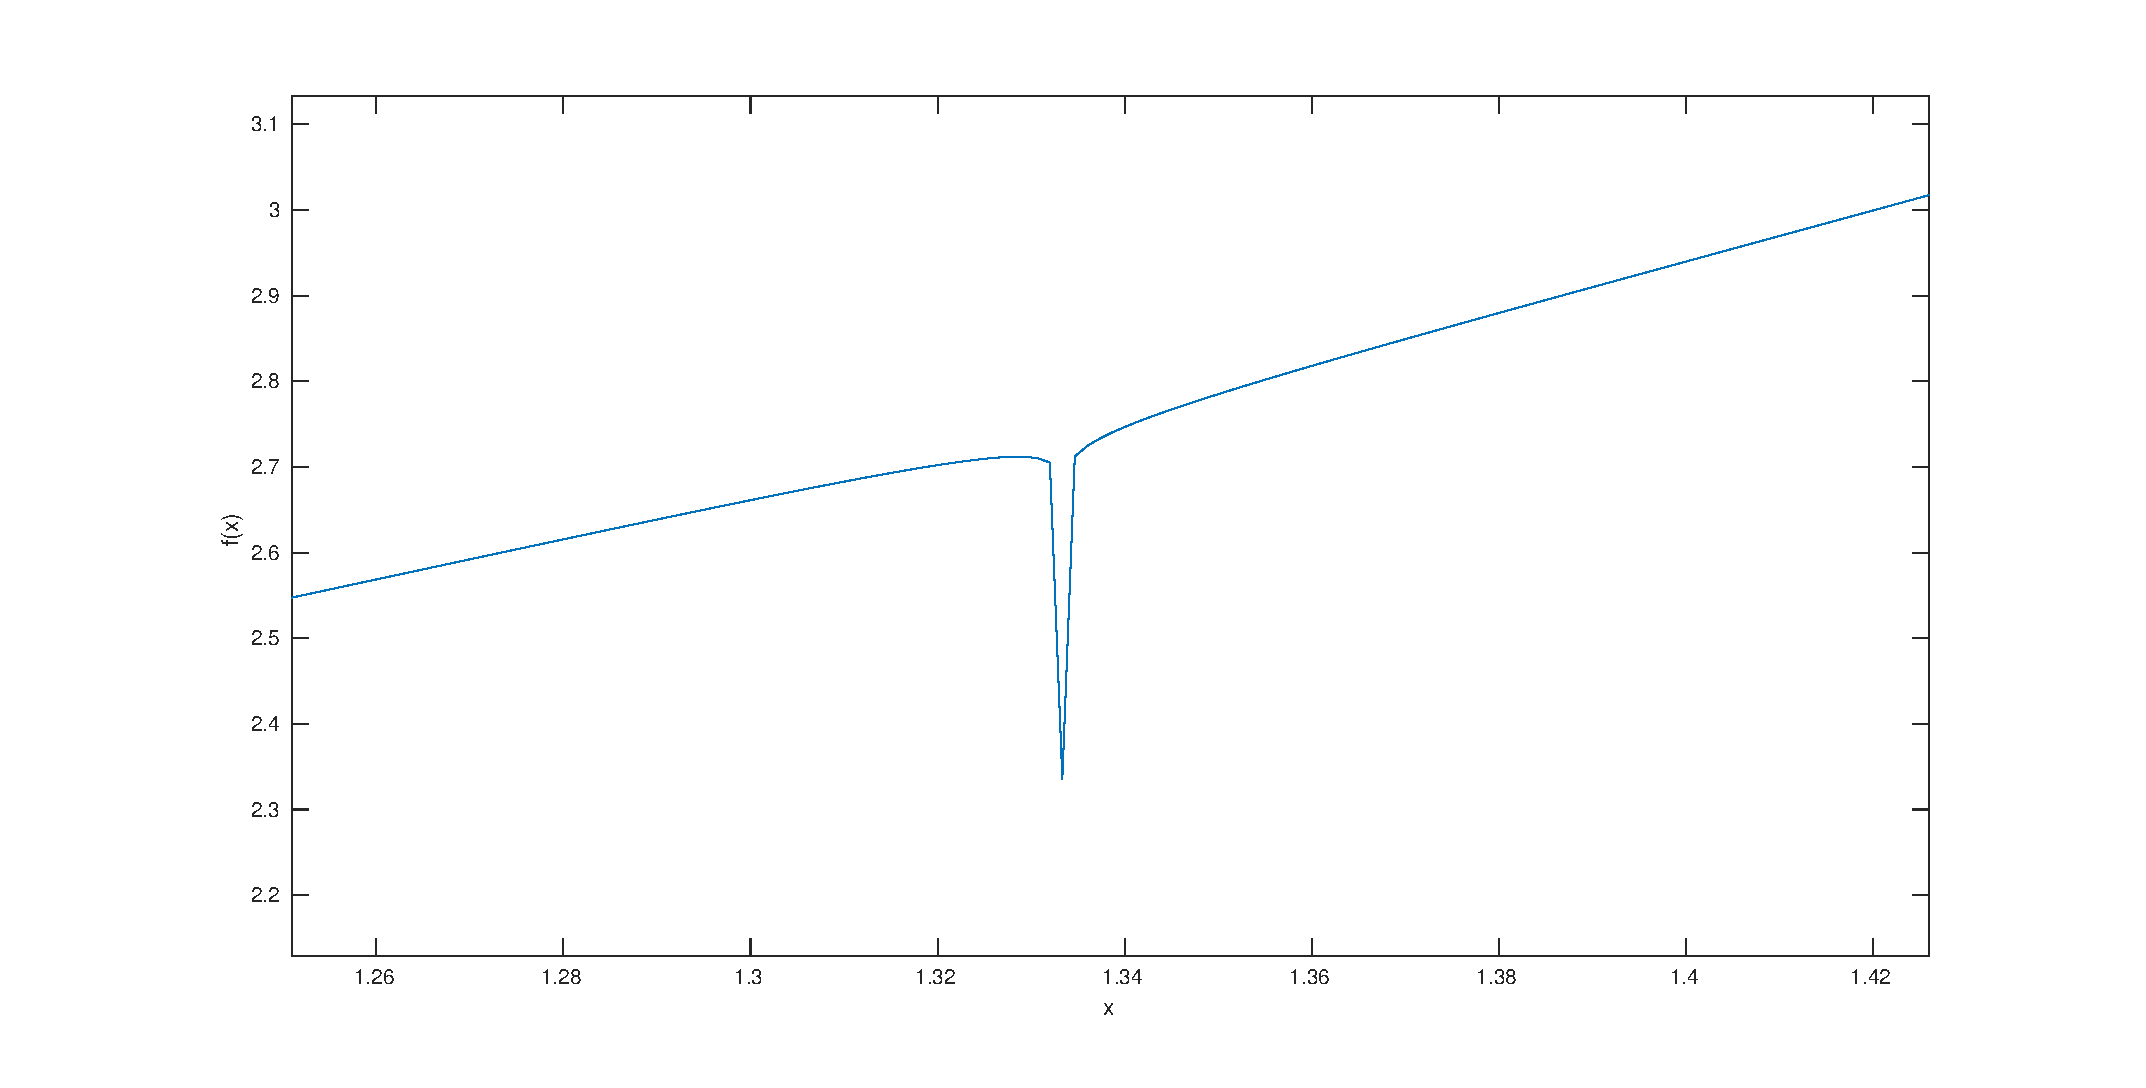
\includegraphics[width=\textwidth]{plot/fes113}
\end{figure}

\end{document}
